\chapter{Initialisierung}

\label{ReportInitialisierung}

\section{Ausgangslage}

Als regelmässiger Konzertbesucher wünsche ich mir eine Plattform im
Internet, auf welcher ich eine zuverlässige Übersicht an Konzerten in
meiner Umgebung vorfinde. Heute sind die Events nur verteilt auf
verschiedenen Seiten wie die der Venues, des Konzertveranstalters, des
Künstlers oder auf Facebook publiziert.\\

\noindent
Ich möchte deshalb eine zentrale Plattform entwickeln, die es Benutzern
einfach macht, Konzerte für ihren Geschmack zu finden.
Die Plattform soll Genre unabhängig sein und entsprechende Filter anbieten.
Den Benutzern der Plattform soll es möglich sein, Konzerte selber zu
erfassen und pflegen.\\

\noindent
Um einen zusätzlichen Service für den Benutzer zur Verfügungs zu stellen,
ist es auch denkbar, eine Art Notifikationssystem zu bauen um Benutzer
über Handy-Notifications oder per Email an Konzerte oder Künstler zu
erinnern.\\

\noindent
Konzertveranstaltern kann das Erfassen ihrer Events vereinfacht werden,
indem auf der Plattform erfasste Veranstaltungen direkt auf den Sozialen
Medien wie Facebook, Twitter oder Instagram geteilt werden können.


\clearpage
\section{Projektziele}

Folgende Ziele sind in der Initialisierungsphase definiert worden:

\begin{longtable}[]{@{}lll@{}}
  \toprule
  Nr.  & Zielbeschreibung                                                                       & Muss/Kann\tabularnewline
  \toprule
       & Produktziele\tabularnewline
  \midrule
  1.1  & Besucher können im Produkt nach Konzerten suchen                                       & Muss\tabularnewline
  1.2  & Suchresultate können nach Musik-Genre und Ort gefiltert werden                         & Muss\tabularnewline
  1.3  & Das Produkt soll ein modernes responsives Design vorweisen                             & Muss\tabularnewline
  1.4  & Konzerte sollen von Suchmaschinen indexiert werden können                              & Muss\tabularnewline
  1.5  & Benutzer können isch im Produkt registrieren                                           & Muss\tabularnewline
  1.6  & Benutzer können ihr Passwort nach Verlust neu setzen                                   & Muss\tabularnewline
  1.7  & Inhalte des Portals sind durch die Benutzer erfassbar und bearbeitbar                  & Muss\tabularnewline
  1.8  & Kompatibilität mit aktuellem Google Chrome und Mozilla Firefox Browser                 & Muss\tabularnewline
  1.9  & Konzerte können vom Produkt nach Facebook exportiert werden                            & Kann\tabularnewline
  1.10 & Ein angemeldeter Benutzer kann vermerken ob er einem Konzert teilnimmt                 & Kann\tabularnewline
  1.11 & Das Produkt soll sich an Security Best-Practices von OWASP halten                      & Muss\tabularnewline
  \bottomrule
       & Abwicklungsziele\tabularnewline
  \midrule
  2.1  & \makecell[l]{Das Projekt soll nach HERMES 5 unter Berücksichtigung der Richtlinien von                            \\ der TSBE dokumentiert werden} & Muss\tabularnewline
  2.2  & Das Produkt muss bis Projektende fertiggestellt und bereit für die Einführung sein     & Muss\tabularnewline
  2.3  & Die Technische-Umsetzung wird durch Damian Senn erstellt                               & Muss\tabularnewline
  2.4  & \makecell[l]{Die Kommunikation zwischen Experten und Diplomanden erfolgt wie im                                   \\ Projektauftrag \ref{kommunikation} beschrieben.} & Muss\tabularnewline
  2.5  & Das Projekt muss bis Ende Mai 2019 abgeschlossen sein                                  & Muss\tabularnewline
  \bottomrule
\end{longtable}


\clearpage

\section{Projektorganisation}

\begin{figure}[!htb]
  \centering
  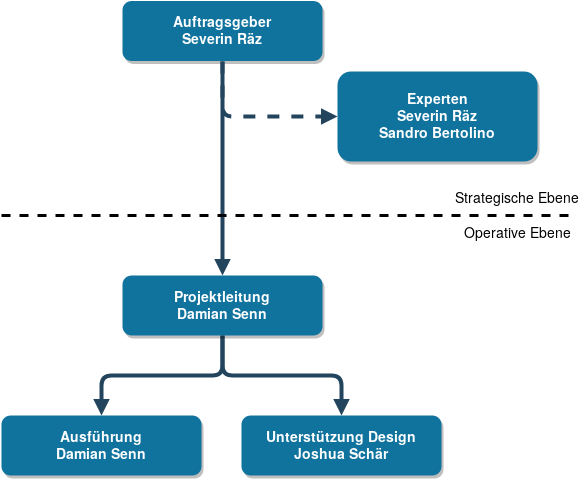
\includegraphics[width=0.8\textwidth]{figures/organigram.png}
  \caption{Organigram}
\end{figure}

\subsection{Tätigkeiten im Projekt}\label{tuxe4tigkeiten-im-projekt}

Für die Freigaben der Phasen ist nach Absprache mit Severin Räz Damian Senn
selbstständig verantwortlich.

\begin{longtable}[]{@{}ll@{}}
  \toprule
  \textbf{Name}    & \textbf{Funktions- und Tätigkeitsbereich}\tabularnewline
  \midrule
  \endhead
  Severin Räz      & Auftraggeber, externer Experte\tabularnewline
  Sandro Bertolino & Interner Experte\tabularnewline
  Damian Senn      & Projektleiter, Ausführung\tabularnewline
  Joshua Schär     & Unterstützung Design\tabularnewline
  \bottomrule
  \caption{Tätigkeiten Verteilung}
\end{longtable}

\subsection{Kommunikation}\label{kommunikation}

Im Kickoff-Meeting wurde besprochen, dass Damian Senn alle zwei Wochen einen
kurzen Bericht an Sandro Bertolino und Severin Räz per E-Mail schicken wird.
Im Bericht soll erläutert werden, was in der Zwischenzeit erledigt wurde und
was die nächsten Schritte im Projekt sind.

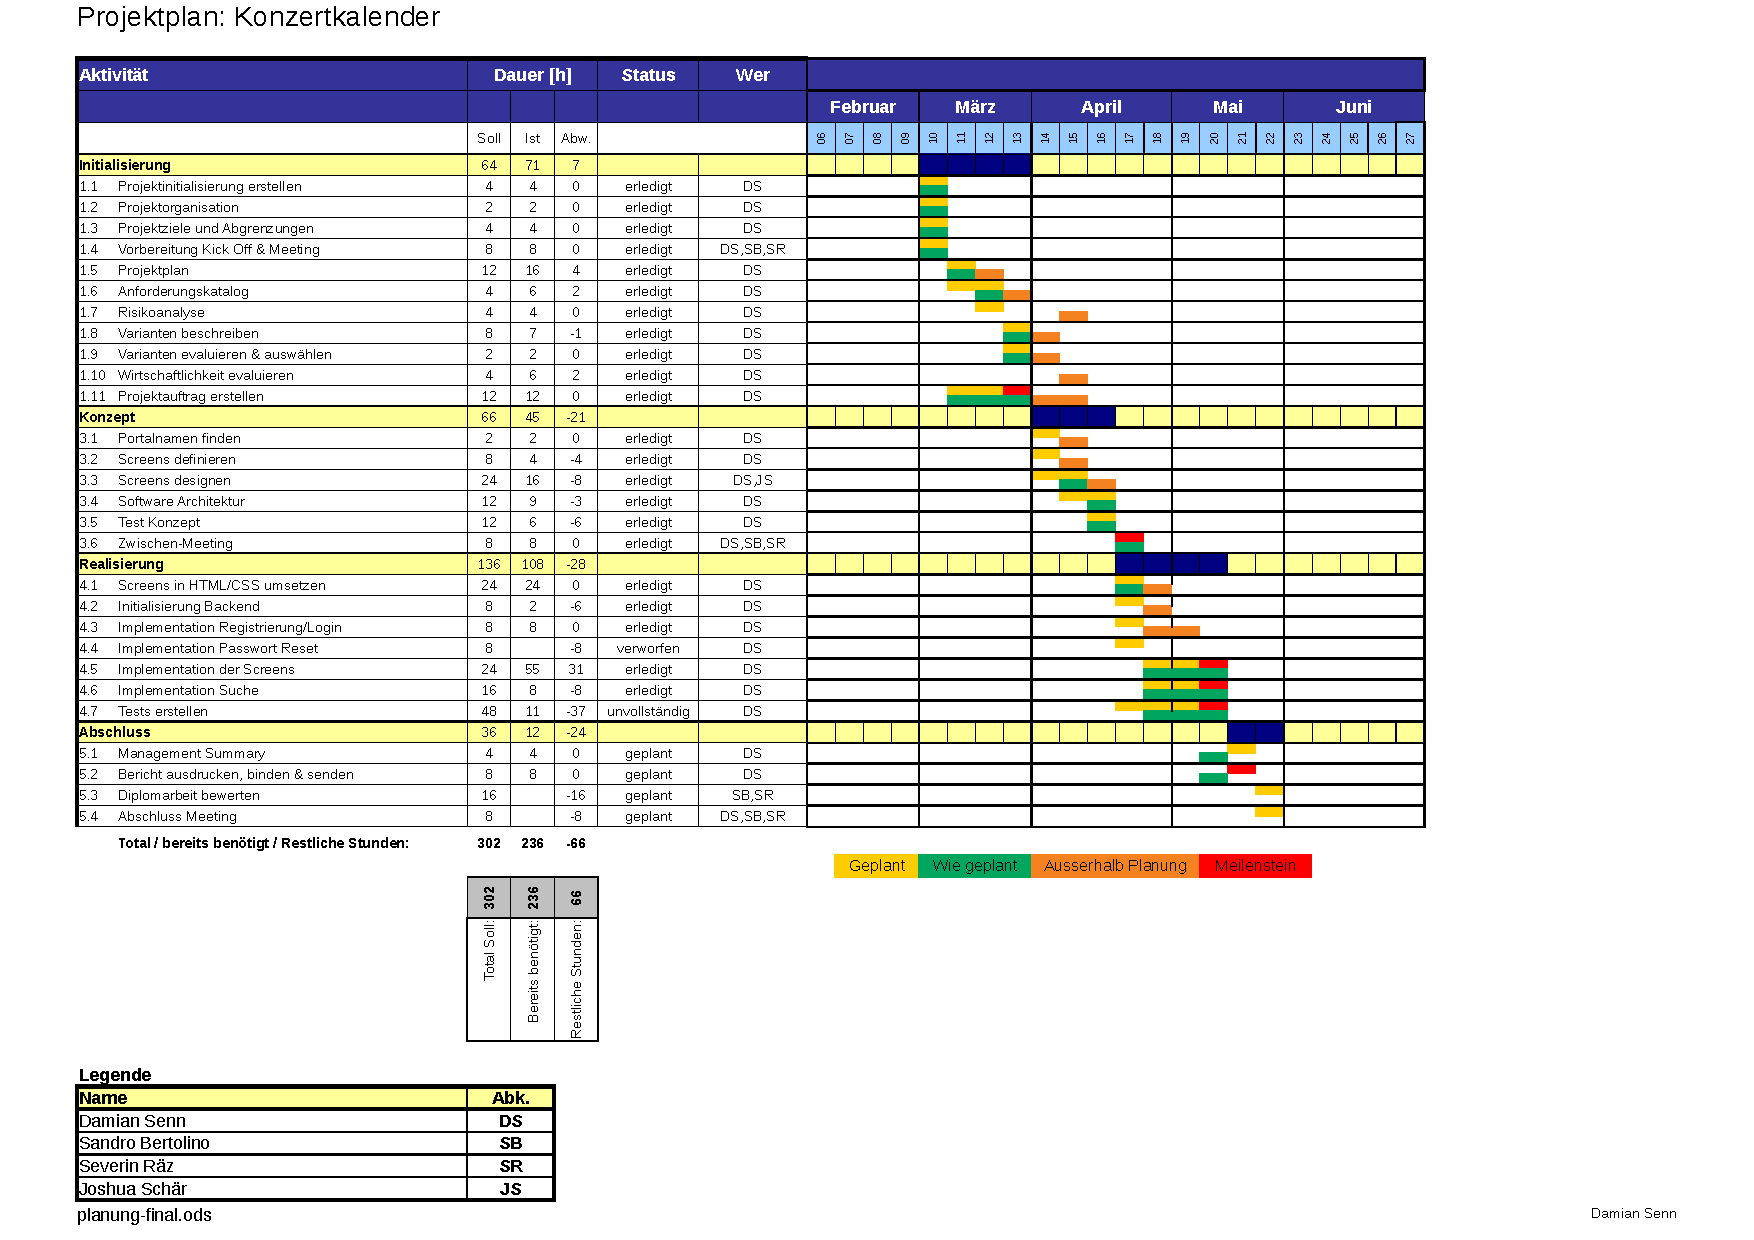
\includepdf[pagecommand={\section{Ausgefüllter Projektplan}}]{figures/planung-final.pdf}

\section{Lieferergebnisse}

Folgende Ergebnisse wurden in der Phase Initialisierung erstellt:

\begin{itemize}
  \tightlist{}
  \item{}Studie (Anhang~\ref{AppendixStudie})
  \item{}Projektauftrag (Anhang~\ref{AppendixProjektauftrag})
\end{itemize}

\section{Terminplan}

Nachfolgend ist der grobe Terminplan der während der Initialisierungsphase
erstellt wurde für die geplanten Phasen.

\begin{longtable}[]{@{}lrr@{}}
  \toprule
  Phase           & Datum                   & Stunden\tabularnewline
  \midrule
  \endhead
  Initialisierung & 06.03.2019 - 31.03.2019 & 64\tabularnewline
  Konzept         & 01.04.2019 - 21.04.2019 & 66\tabularnewline
  Realisierung    & 22.04.2019 - 19.05.2019 & 136\tabularnewline
  Abschluss       & 20.05.2019 - 21.05.2019 & 36\tabularnewline
  \midrule
                  & Total:                  & 302\tabularnewline
  \bottomrule
  \caption{Terminplan}
\end{longtable}

\clearpage
\section{Risiken}

Die Risikobewertung erfolgt mit folgender Formel:\\

\textbf{Bewertung = Schaden x Eintrittswahrscheinlichkeit}\\

\noindent{}Weitere Details zur Bewertung der Risiken sind im Projektauftrag Anhang~\ref{risiken} zu finden.

\subsection{Projektrisiken}\label{projektrisiken}

\begin{longtable}[]{@{}lp{3cm}p{4cm}ccc@{}}
  \toprule
  \textbf{Nr.} & \textbf{Risiko}                             & \textbf{Auswirkung}                                 & \textbf{Schaden} & \textbf{Wahrsch.} & \textbf{Bewertung}\tabularnewline
  \midrule
  \endhead
  1            & Ausfall des Entwicklers oder Projektleiters & Verzögerungen von Arbeiten                          & 4                & 3                 & Mittel\tabularnewline
  2            & Unvollständige Projektdokumentation         & Schlechtere Diplomarbeit Bewertung                  & 4                & 2                 & Mittel\tabularnewline
  3            & Schlechter Projektplan                      & Verzögerungen und eventuelle Qualitätsverluste      & 4                & 3                 & Mittel\tabularnewline
  4            & Keine Benutzer                              & Das Produkt wird nicht von Benutzern eingesetzt     & 3                & 4                 & Mittel\tabularnewline
  5            & Technisch nicht umsetzbare Features         & Das Produkt kann nicht wie angedacht benutzt werden & 4                & 3                 & Mittel\tabularnewline
  \bottomrule
  \caption{Projektrisiken}
\end{longtable}

\clearpage
\subsection{Massnahmen}\label{massnahmen}

\begin{longtable}[]{@{}lp{4.1cm}lccc@{}}
  \toprule
               &                                                                       &                   & \multicolumn{3}{l}{\textbf{Bewertung nach Massnahme}}\tabularnewline
  \textbf{Nr.} & \textbf{Massnahme}                                                    & \textbf{Handlung} & \textbf{Schaden}                                                     & \textbf{Wahrsch.} & \textbf{Bewertung}\tabularnewline
  \midrule
  \endhead
  1            & Arzt aufsuchen, ggf. Projekt-Pause oder Abbruch                       & Akzeptanz         & 4                                                                    & 3                 & Mittel\tabularnewline
  2            & Statusbericht alle zwei Wochen, bei Fragen sofort Hilfe suchen        & Verminderung      & 2                                                                    & 1                 & Gering\tabularnewline
  3            & Genügend Buffer-Zeit einplanen, ggf. Ferientage für Projekt einsetzen & Verminderung      & 2                                                                    & 1                 & Gering\tabularnewline
  4            & Das Produkt löst vor allem ein persönliches Interesse                 & Akzeptanz         & 3                                                                    & 4                 & Mittel\tabularnewline
  5            & Vereinfachte Alternativen in Konzept-Phase untersuchen                & Verminderung      & 2                                                                    & 2                 & Gering\tabularnewline
  \bottomrule
  \caption{Projektrisiken - Massnahmen}
\end{longtable}

\subsection{Risikodiagramm}

Die Risikodiagramme sind im Projektauftrag im Anhang~\ref{risikodiagram-ohne-massnahmen} und Anhang~\ref{risikodiagram-mit-massnahmen} zu finden.

\clearpage

\section{Abgrenzungen}

\begin{figure}[!htb]
  \centering
  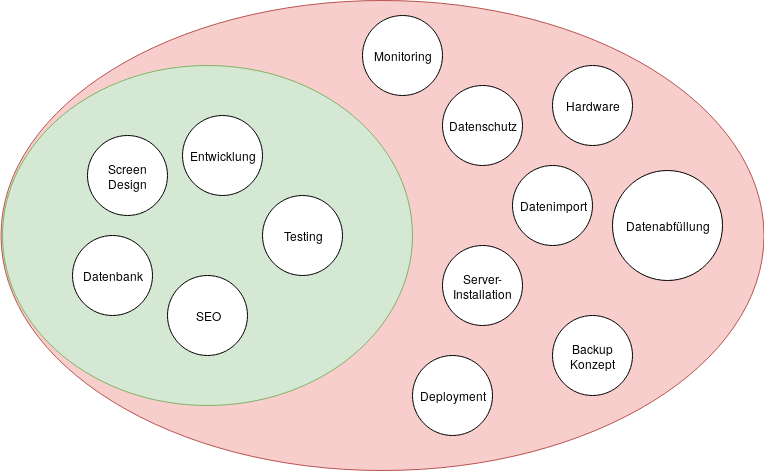
\includegraphics[width=0.95\textwidth]{figures/abgrenzungen.png}
  \caption{Abgrenzungen}
\end{figure}

\noindent
Die detaillierten Erklärung zu den einzelnen Abgrenzungen sind im Projektauftrag~\ref{abgrenzungen} zu finden.

\clearpage

\section{Studie}

In der Studie wurden folgende Arbeiten abgehandelt:

\begin{itemize}
  \tightlist
  \item der Anforderungskatalog wurde definiert
  \item die Evaluation der Browser Software-Technologien
  \item die Evaluation der Server Software-Technologien
  \item die Evaluation der Testing Software-Technologien
  \item eine Kostenschätzung und mögliche Wirtschaftlichkeit ausgerechnet
\end{itemize}

\subsection{Informationsbeschaffung}

Folgende Quellen wurden in diesem Projekt für die Informationsbeschaffung
genutzt:

\begin{longtable}[]{@{}p{3cm}p{10cm}@{}}
  \toprule
  \textbf{Quelle}               & \textbf{Beschreibung}\tabularnewline
  \toprule
  Schulwissen / Berufserfahrung & Die Grundlage für die Umsetzung dieses Projekts wird durch mein existierendes Schulwissen sowie meine langjährige Berufserfahrung in der Software-Entwicklung gesetzt.\tabularnewline
  \midrule
  Internet                      & Ein Grossteil der Informationen werden heute über das Internet bezogen, für die Evaluation von Technologien und Lösungsansätzen wird einiges über das Internet recherchiert werden müssen.\tabularnewline
  \midrule
  Externer Experte              & Bei konzeptionellen sowie technischen Fragen kann der externe Experte um Rat gefragt werden.\tabularnewline
  \bottomrule
  \caption{Informationsbeschaffung}
\end{longtable}


\clearpage
\subsection{Anforderungskatalog}

Im Anforderungskatalog werden die Muss- und Kann-Kriterien definiert.
Muss-Kriterien sind zwingend zu erfüllen, Kann-Kriterien sind als optionale
Erweiterung zu verstehen.

% TODO: Fix multirows across pages
%       https://tex.stackexchange.com/questions/79143/how-to-repeat-cell-content-on-next-page-for-longtable-using-multirow/79152
\begin{longtable}[]{@{}p{1.9cm}p{2.5cm}cp{5.5cm}cc@{}}
  \toprule
  \textbf{Feature}           & \textbf{Titel}             & \textbf{Nr.} & \textbf{Kriterium}                                                                                          & \textbf{Ziel} & \textbf{Muss}\tabularnewline
  \midrule
  \endhead
  \multirow{10}{*}{Suche}    & Suche nach Konzertname     & 1.1          & Listet alle Konzerte die Wörter der Suche im Konzertnamen beinhalten                                        & 1.1           & \textbf{Muss}                \\ \cline{2-6}
                             & Suche nach Konzertlocation & 1.2          & Schränkt die Such-Resultate nach gegebener Konzertlocation ein                                              & 1.2           & \textbf{Muss}                \\ \cline{2-6}
                             & Suche nach Ort             & 1.2          & Schränkt die Such-Resultate nach gegebenem Ort ein                                                          & 1.2           & \textbf{Muss}                \\ \cline{2-6}
                             & Suche nach Genre           & 1.2          & Schränkt die Such-Resultate nach gegebenem Musik-Genre ein                                                  & 1.2           & \textbf{Muss}                \\
  \midrule
  \multirow{8}{*}{Design}    & Desktop                    & 2.1          & Alle Ansichten haben eine Desktop-Optimierte Variante                                                       & 1.4           & \textbf{Muss}                \\ \cline{2-6}
                             & Tablet                     & 2.2          & Alle Ansichten haben eine Tablet-Optimierte Variante                                                        & 1.4           & \textbf{Muss}                \\ \cline{2-6}
                             & Mobile                     & 2.3          & Alle Ansichten haben eine Mobile-Optimierte Variante                                                        & 1.4           & \textbf{Muss}                \\ \cline{2-6}
                             & Browser Kompatibilität     & 2.4          & Alle Ansichten müssen in aktuellem Google Chrome und Mozilla Firefox dem Grundlayout folgen                 & 1.9           & \textbf{Muss}                \\
  \midrule
  \multirow{4}{*}{SEO}       & Indexierbarkeit            & 3.1          & Das Produkt ist von Suchmaschinen indexierbar                                                               & 1.5           & \textbf{Muss}                \\ \cline{2-6}
                             & Linked Data                & 3.2          & Konzert Detailseiten sind mit dem Event-Schema\footnote{\url{https://schema.org/Event}} ausgestattet              & 1.5           & \textbf{Muss}                \\
  \midrule
  \multirow{8}{*}{Benutzer}  & Registrierung              & 4.1          & Besucher können sich einen Benutzer registrieren, Benutzernamen und E-Mail Adressen müssen einzigartig sein & 1.6           & \textbf{Muss}                \\ \cline{2-6}
                             & Passwort-Vergessen         & 4.2          & Benutzer können sich einen Passwort-Reset Link anfordern                                                    & 1.7           & \textbf{Muss}                \\ \cline{2-6}
                             & Social                     & 4.3          & Benutzer können auf Konzerten vermerken ob sie Teilnehmen oder nicht                                        & 1.11          & Kann                         \\
  \midrule
  \clearpage
  \multirow{6}{*}{Erfassung} & Artist                     & 5.1          & Benutzer können Artisten mit einem Genre erfassen                                                           & 1.8           & \textbf{Muss}                \\ \cline{2-6}
                             & Location                   & 5.2          & Benutzer können eine Konzertlocation mit Ort/Strasse erfassen                                               & 1.8           & \textbf{Muss}                \\ \cline{2-6}
                             & Konzert                    & 5.3          & Benutzer können ein Konzert mit Konzertlocation und Artisten erfassen                                       & 1.8           & \textbf{Muss}                \\ \cline{2-6}
                             & Facebook                   & 5.4          & Benutzer können ein Konzert in ein Facebook-Event exportieren                                               & 1.10          & Kann                         \\
  \midrule
  \multirow{9}{*}{Security}  & SQL-Injection              & 6.1          & Das Produkt soll resistent gegen SQL-Injection sein                                                         & 1.12          & \textbf{Muss}                \\ \cline{2-6}
                             & HTML-Injection             & 6.2          & Das Produkt soll resistent gegen HTML-Injection / XSS sein                                                  & 1.12          & \textbf{Muss}                \\ \cline{2-6}
                             & Passwort encryption        & 6.3          & Passwörter von Benutzer müssen mit einem sicheren Verfahren gespeichert werden                              & 1.12          & \textbf{Muss}                \\ \cline{2-6}
                             & Session                    & 6.4          & Session-Cookies dürfen nicht durch JavaScript ausgelesen werden                                             & 1.12          & Kann                         \\
  \midrule
  Performance                & Ladezeit                   & 7.1          & Die Seitenansichten dürfen nicht länger als 6 Sekunden auf einem 3G Netz laden                              &               & \textbf{Muss}                \\
  \midrule
  Sonstiges                  & User Tracking              & 8.1          & Benutzerverhalten soll analysiert und nachvollziehbar sein.                                                 &               & Kann                         \\
  \bottomrule
  \caption{Anforderungskatalog}
\end{longtable}


\clearpage
\section{Evaluation Browser-Technologie}

\noindent{}Die genaue Erklärung zur Gewichtung der Browser-Technologie
Evaluation sind in der Studie im Anhang~\ref{evaluation-browser-technologie}
zu finden.

\subsection{Variante: React}

Die JavaScript Library \textbf{React} ist heute die wohl beliebteste
Technologie um interaktive Applikationen im Web zu bauen.

React ermöglicht es den Entwicklern Screens auf eine deklarative Weise zu
definieren, so dass sich Elemente jeweils dem Zustand der Applikation anpassen.

Die Features von React sind minimal gehalten und sehen auf den ersten Blick
einfach aus, jedoch wird für Anwendungen schnell klar, dass zusätzliche
Software-Libraries benötigt werden um eine grössere Applikation zu entwickeln.

Durch das Hinzufügen von weiteren Libraries steigt die Komplexität dieser
Variante stark an, da es im React Ökosystem für viele Lösungen diverse
verschiedene Lösungsansätze gibt.

\subsection{Variante: Next.js}

\textbf{Next.js} ist ein JavaScript Framework, das auf der \textbf{React}
Library aufbaut und zusätzliche Features sowie gängige Konventionen mitbringt.

Dadurch dass Next.js ein komplettes Framework ist und nicht nur eine Library,
leidet diese Variante weniger der Komplexität eines kompletten Eigenbaus mit
React. Features wie die Navigation von Seite zu Seite bringt Next.js bereits
mit.

\subsection{Variante: SSR}

\textbf{SSR} steht für \textbf{S}erver\textbf{s}ide \textbf{R}endering und
beschreibt die klassische Methode vom Erstellen von Webseiten, indem man HTML
auf dem Server generiert und zum Browser schickt.

Dies hat nach wie vor seine Daseinsberechtigung, da dies wenig Komplexität
mit sich bringt, einen schnelleren Seitenaufbau garantiert und ohne
zusätzlichen Aufwand von Suchmaschinen indexiert werden kann.

\section{Entscheid Browser-Technologie}\label{entscheid-browser-technologie}

Die Bewertung der Browser-Technologie sind in der Studie im
Anhang~\ref{bewertungen-browser-technologie} zu finden.

Durch die Evaluierung wurde klar, dass das Einsetzen eines JavaScript-Frameworks
zuviel zusätzliche Komplexität und gewisse Einbussungen in Performance und Stabilität
unvermeidbar ist. Somit ist ein die Wahl für eine klassische Server-Side Rendered
Webseite favorisierend.

Es ist durchaus vorstellbar, dass in einem zweiten Schritt, nach diesem Projekt,
die Server-Side Rendered Applikation durch eine Next.js Applikation ersetzt werden
könnte.

\subsubsection{Kosten / Wirtschaftlichkeit}

Da die Programmiersprache Elixir sowie das Framework Phoenix unter einer
Open Source Lizenz verfügbar sind, fallen bei dieser Lösung keine zusätzlichen
Kosten an.

\clearpage
\section{Evaluation Server-Technologie}\label{evaluation-server-technologie}

\noindent{}Die genaue Erklärung zur Gewichtung der Server-Technologie
Evaluation sind in der Studie im Anhang~\ref{evaluation-server-technologie}
zu finden.

\subsection{Variante: Node.js / koa.js}

Auch auf dem Server gewinnt JavaScript immer mehr an Beliebtheit.
Mit Node.js und koa.js können schnell kleinere und simplere Applikationen
erstellt werden, die dennoch sehr performant sind.

koa.js ist eine Library für Server-Applikationen und bietet nur eine einfache
Basis und bringt keine Features für Datenpersistenz oder HTML Templates mit sich.
Diese Features müssen durch zusätzliche Module installiert werden.

\subsection{Variante: Elixir / Phoenix}

Elixir ist eine Programmiersprache die eine sehr stabile und performante Grundlage
bietet. Durch das Framework Phoenix, wird im Elixir Ökosystem ein starkes feature
umfangreiches Web-Framework angeboten. Phoenix beinhaltet eine grosse Menge an
Features mit sich und gibt dem Entwickler direkt Funktionalitäten wie HTML
Templates, Datenpersistenz und ein einfaches Test-Framework.

\subsection{Variante: Next.js}

Next.js wurde bereits als Variante für die Browser-Technologie in Betracht
gezogen. Ein zusätzliches Feature von Next.js ist, dass die Applikation auch
auf dem Server betrieben werden kann.
Das Einsetzen der selben Technologie kann bedeutende Vorteile mit sich bringen,
so muss man nur ein Framework lernen und kann Programmcode auf dem Server mit
der Applikation im Browser geteilt werden.

\section{Entscheid Server-Technologie}\label{entscheid-server-technologie}

Die Bewertung der Server-Technologie sind in der Studie im
Anhang~\ref{bewertungen-server-technologie} zu finden.

Durch das grosse Featurset von Phoenix sowie tieferer Komplexität gegenüber den
beiden anderen Varianten hat sich Phoenix für die Server-Technologie klar
durchgesetzt.

\subsubsection{Kosten / Wirtschaftlichkeit}

Da die Programmiersprache Elixir sowie das Framework Phoenix unter einer
Open Source Lizenz verfügbar sind, fallen bei dieser Lösung keine zusätzlichen
Kosten an.

\clearpage
\section{Evaluation Testing-Technologie}\label{evaluation-testing-technologie}

\noindent{}Die genaue Erklärung zur Gewichtung der Testing-Technologie
Evaluation sind in der Studie im Anhang~\ref{evaluation-testing-technologie}
zu finden.

\subsection{Jest + Puppeteer}

Jest ist ein JavaScript-Test Framework von Facebook. Durch die Kombinierung der
Puppeteer Library von Google ist es möglich, automatisierte Browser-Tests
durchzuführen.

\subsection{Wallaby}

Wallaby ist ein Elixir Browser-Test Framework, welches sich nahtlos mit Phoenix
integrieren lässt. Wallaby unterstützt parallelisierung von Tests und ist daher
ein guter Kanditat eine hohe Anzahl von automatisierten Tests.

\section{Entscheid Testing-Technologie}\label{entscheid-testing-technologie}

Die Bewertung der Testing-Technologie sind in der Studie im
Anhang~\ref{bewertungen-testing-technologie} zu finden.

Dadurch dass sich Wallaby einfach mit der ausgewählten Server-Technologie
verwenden lässt, hohe Performance und Stabilität aufweist, ist Wallaby die
knapp bessere Variante als eine Jest + Puppeteer kombination.

Leider hat Wallaby keine Visualtesting Integration mit dem Dienst percy.io,
dies könnte aber im verlaufe der Umsetzung eventuell im Rahmen dieser Arbeit
umgesetzt werden.

\subsubsection{Kosten / Wirtschaftlichkeit}\label{WallabyPercy}

Auch Wallaby ist unter eines Open Source Lizenz veröffentlicht und erzeugt
somit im Projekt keine direkten zusätzlichen Kosten. Durch fehlende
Unterstützung von Visualtesting, wird im Verlauf der Realisierung zusätzlicher
Aufwand erzeugt, entweder durch eigene Implementation solcher Tests oder durch
unbemerkte Fehler die sich bei Änderungen eingeschlichen haben.

\clearpage
\section{Wirtschaftlichkeit}\label{wirtschaftlichkeit}

\subsection{Projektkosten}

Für die Berechnung der Projektkosten wird ein Stundensatz von 150.- CHF angenommen.

\begin{longtable}[]{@{}lrr@{}}
  \toprule
  \textbf{Phase}  & \makecell[r]{\textbf{Geplante} \\\textbf{Stunden}} & \textbf{Kosten}\tabularnewline
  \midrule
  \endhead
  Initialisierung &  64                       &  9'600.- CHF\tabularnewline
  Konzept         &  66                       &  9'900.- CHF\tabularnewline
  Realisierung    & 136                       & 20'400.- CHF\tabularnewline
  Abschluss       &  64                       &  5'400.- CHF\tabularnewline
  \midrule
  \textbf{Total:} & 286                       & 42'900.- CHF\tabularnewline
  \bottomrule
  \caption{Projektkosten}
\end{longtable}


\noindent
Die geplanten Projektkosten betragen somit \textbf{42'900.- CHF}.

\begin{longtable}[]{@{}lll@{}}
  \toprule
  \textbf{Kostenstelle} & \textbf{Jährliche Kosten}\tabularnewline
  \midrule
  \endhead
  Software              & Keine\tabularnewline
  .com Domain           & 20.- CHF\tabularnewline
  Hosting               & 1'800.- CHF\tabularnewline
  \midrule
  \textbf{Total:}       & 1'820.- CHF\tabularnewline
  \bottomrule
  \caption{Betriebskosten}
\end{longtable}


Für die Betriebskosten eines Hostings wird einen durchschnittlichen monatlichen
Preis von 150.- CHF angenommen, da das Deployment für dieses nicht vorgesehen
ist, ist dies eine von Damian Senn geschätzte Zahl.

\clearpage
\subsection{Break Even Analyse}\label{break-even-analyse}

Beim Modell «Gigboost» wird eine Option angeboten bei der publizierten Gigs auf
der Startseite sowie in der Suche anderen Einträgen bevorzugt dargestellt
werden. Für einen Gegenpreis von 10.- CHF kann man einen Gig «boosten».

\begin{figure}[!htb]
  \centering
  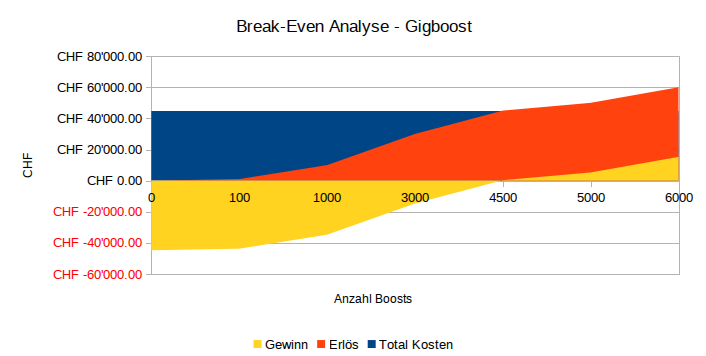
\includegraphics[width=0.95\textwidth]{initialisierung/wirtschaftlichkeit-gigboost.png}
  \caption{Break-Even Analyse - Gigboost}
\end{figure}

Im Modell «Werbung» wird ausgerechnet wieviele aktive Benutzer das Produkt benötigt
um in den nächsten Jahren Gewinn zu erzielen.

Durch Annahme von einem Erlös von \textbf{140.- CHF} pro \textbf{40'0000 Besucher}\footnote{\url{https://www.quora.com/How-much-does-Google-AdSense-pay-for-3-banners-on-a-webpage-per-1-000-views/answer/Manas-Sahu-59}} erhalten wir folgendes Bild:

\begin{figure}[!htb]
  \centering
  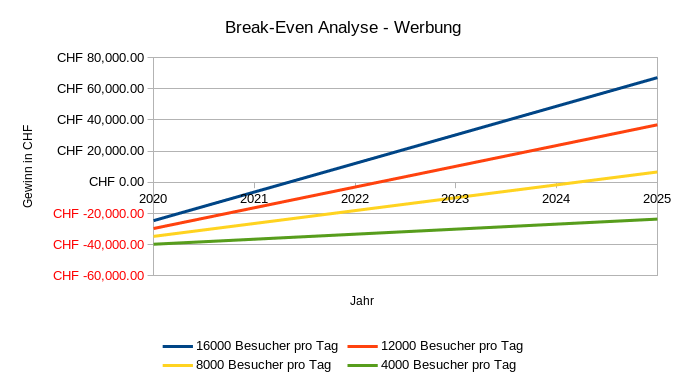
\includegraphics[width=0.95\textwidth]{initialisierung/wirtschaftlichkeit-werbung-updated.png}
  \caption{Break-Even Analyse - Werbung}
\end{figure}

Die genauere Ausrechnung der Wirtschaftlichkeit im Modell Werbung sind in der
Studie im Anhang~\ref{break-even-analyse-werbung} zu finden.
